\documentclass[12pt,oneside]{amsart}

\title{MATH 536 Project 1}
\author{James Rushing}
\date{02/07/20}

% Homework template by Zach Teitler
% Public domain, free to use and modify for any purpose
% v1.0 2020-01-13

% Packages

\usepackage[T1]{fontenc}
\usepackage{amsmath,amsfonts,amssymb,amsthm}
\usepackage[letterpaper,margin=1.5in]{geometry}
\usepackage[pagebackref]{hyperref}
\usepackage{booktabs}
\usepackage{enumitem}
\usepackage{pgfplots}
\usepgfplotslibrary{polar}
\usepgflibrary{shapes.geometric}
\usetikzlibrary{calc}


\usepackage{fancyhdr}
\pagestyle{fancy}



% Extra space between lines

\linespread{1.5}



% Theorems, lemmas, etc.


\newtheorem{theorem}[equation]{Theorem}
\newtheorem{claim}[equation]{Claim}
\newtheorem{lemma}[equation]{Theorem}
\newtheorem{corollary}[equation]{Theorem}
\newtheorem{conjecture}[equation]{Conjecture}
\newtheorem{question}[equation]{Question}

\theoremstyle{definition}

\newtheorem{definition}[equation]{Definition}

\theoremstyle{remark}

\newtheorem{exer}{Exercise}
\newtheorem{remark}[equation]{Remark}
\newtheorem{example}[equation]{Example}

\numberwithin{equation}{exer}


% Answers

% Use "proof" for proof exercises!
% Use "answer" for question (non-proof) exercises

\newenvironment{answer}{\bigskip\noindent\emph{Answer.}}{\hfill$\diamond$\newline}


% Symbols

\newcommand{\bbC}{\mathbb{C}}
\newcommand{\bbN}{\mathbb{N}}
\newcommand{\bbR}{\mathbb{R}}
\newcommand{\bbQ}{\mathbb{Q}}
\newcommand{\bbZ}{\mathbb{Z}}




\begin{document}
\maketitle

\begin{exer} (Problem 3 Page 3)
\\\newline
Solve $(x-1)y'+ 2y =x$, where $x\neq1$
\end{exer}

\begin{answer}
\begin{align*}
    (x-1)y'+ 2y =x \\
 \implies y' +\left(\frac{2}{x-1}\right)(y) = \frac{x}{x-1} 
\end{align*}
\newline
Where $p(x) = \frac{2}{x-1}$. Now using the integration factor 
\newline
\begin{align*}
    u(x) =  exp\Big\{\int p(x)dx\Big\}=exp\Big\{\int \frac{2}{x-1}dx\Big\} = exp\Big\{2ln(x-1)\Big\} = (x-1)^2
\end{align*}
\newline
We have
\begin{align*}
    y' + \left(\frac{2}{x-1}\right)y = \frac{x}{x-1}\Bigg|\cdot  (x-1)^2\\
    \implies y'(x-1)^2 + 2y(x-1) = x(x-1) \\
    \implies  y'(x-1)^2 + y((x-1)^2)' = x^2-x.
\end{align*}
\newline
Reversing the product rule and integrating gives us
\begin{align*}
    \int (y(x-1)^2)' = \int (x^2 - x)\\
    \implies y  (x-1)^{2}= \frac{x^3}{3} -\frac{x^2}{2} + C\\
    \implies y = (x-1)^{-2}\Big[\frac{x^3}{3} -\frac{x^2}{2} + C\Big].
\end{align*}

\end{answer}


\newpage
\begin{exer} (Problem 5 page 6)
Solve $4y'' + 4y' +y = 0$.
\end{exer}

\begin{answer}
Given a second-order differential equation with constant coefficients, we can write 
\begin{align*}
    y = e^{\lambda x } \indent y' = \lambda e^{\lambda x } \indent y''= \lambda^2e^{\lambda x}.
\end{align*}
With this, our equation becomes $4\lambda^2e^{\lambda x} + 4 \lambda e^{\lambda x} +e^{\lambda x} = 0$ and our characteristic equation is as follows:
\begin{align*}
    4\lambda^2 + 4 \lambda  +1 = 4\lambda^2 + 2\lambda + 2\lambda +1 = 2\lambda(2\lambda +1)+(2\lambda +1) \\
    =(2\lambda +1)(2\lambda +1) = (2\lambda+1)^2 = 0.
\end{align*}
From this we can conclude that our characteristic equation has a double root at $\lambda = - \frac{1}{2}$. Finally we can write the following solutions and combine them into a general solution:
\begin{align*}
    y_1(x) = e^{-\frac{x}{2}} \indent y_2(x) = x e^{-\frac{x}{2}}\\
    \implies y(x) = C_1 e^{-\frac{x}{2}} + C_2  x e^{-\frac{x}{2}}.
\end{align*}
\end{answer}

\newpage



\begin{exer} (Problem 7 page 8) \\
\newline
Find the general solution of $y'' - 25y = 30 e^{-5x}$.
\end{exer}

\begin{answer}
To find the general solution of $y(x)$ we will find a general solution of it's homogeneous counterpart and combine it with a particular solution of $y(x)$. First we write 
\begin{align*}
    y = e^{\lambda x } \indent y' = \lambda e^{\lambda x } \indent y''= \lambda^2e^{\lambda x}.
\end{align*}
This gives us 
\begin{align*}
    \lambda^2 e^{\lambda x} + 25 e^{\lambda x} = 0 \\
   \implies (\lambda ^2 - 25) = 0 \\
   \implies \lambda = \pm 5 .
\end{align*}
Now we have $y_h(x) = C_1 e^{-5x} + C_2 e^{5x}$. To give ourselves a chance to find a particular solution, we say 
\begin{align*}
    y_p(x)=Axe^{-5x} \\
    y'_p(x) = A(e^{-5x}-5xe^{-5x})\\
    y''_p(x) = A[-5e^{-5x} - 5(e^{-5x} -5xe^{-5x})] \\
    = A(-5e^{-5x} - 5e^{-5x} +25xe^{-5x})\\
    =A(-10e^{-5x} + 25xe^{-5x}).
\end{align*}
Plugging these into our original equation and solving for $A$ gives us the following:
\begin{align*}
    y'' - 25y = -10Ae^{-5x} + 25Axe^{-5x} - 25Axe^{-5x} = -10Ax = 30e^{-5x} \\
    \implies A=-3.
\end{align*}
\indent \newline
Combining gives a general solution of
\begin{align*}
    y(x)=y_h(x) + y_p(x) = C_1 e^{-5x} + C_2 e^{5x} - 3 x e^{-5x}.
\end{align*}
\end{answer}
\newpage
\begin{exer}

\end{exer}
\begin{answer}
The coefficients of the Fourier series are
\begin{align*}
    a_0 = \frac{1}{2L} \int_{-L}^{L}x dx = \frac{1}{2L}\Bigg[\frac{x^2}{2}\Bigg]_{-L}^{L} = 0\\
    a_n = \frac{1}{L} \int_{-L}^{L} x \cos\Big(\frac{n \pi x}{L}\Big)dx = 0
\end{align*}
The function $ x \cos\Big(\frac{n \pi x}{L}\Big)$ is an odd function because it is an odd function times an even function. We are integrating this function symmetrically across the origin so $a_n = 0$. And finally, using integration by parts
\begin{align*}
    b_n = \frac{1}{L}\int_{-L}^{L} x \sin\Big( \frac {n \pi x}{L} \Big) dx = \frac{1}{L} \int_{-L}^{L} x \Big[-\frac{L}{n \pi} \cos\Big(\frac{n \pi x}{L} \Big)\Big]'dx\\
    = \frac{1}{L} \Bigg[ \Big[ x [-\frac{L}{n \pi} \cos\Big(\frac{n \pi x}{L} \Big)]\Big]_{-L}^{L} - \int_{-L}^{L} -\frac{L}{n \pi} \cos\Big(\frac{n \pi x}{L} \Big)dx \Bigg]\\
     = \frac{1}{L} \Bigg[ \Big[ x [-\frac{L}{n \pi} \cos\Big(\frac{n \pi x}{L} \Big)]\Big]_{-L}^{L} + \frac{L}{\pi n}\Big[\frac{L}{\pi n}\sin\Big(\frac{n \pi x}{L}\Big) \Big]_{-L}^{L}\Bigg] \\
     = \frac{1}{L} \Bigg[\Big[ x [-\frac{L}{n \pi} \cos\Big(\frac{n \pi x}{L} \Big)]\Big]_{-L}^{L} + \frac{L^2}{\pi^2n^2}\Big[\sin{n \pi}\Big]\Bigg] \\
     = \frac{1}{L} \Big[ x [-\frac{L}{n \pi} \cos\Big(\frac{n \pi x}{L} \Big)]\Big]_{-L}^{L} + 0 \\
     =\frac{1}{L} \Big[ L [-\frac{L}{n \pi} \cos\Big(\frac{n \pi L}{L} \Big)]- (-L) [-\frac{L}{n \pi} \cos\Big(\frac{n \pi (-L)}{L} \Big)]\Big]\\
    =-\frac{L}{n \pi} \cos(n \pi ) -\frac{L}{n \pi} \cos(n \pi ) = -\frac{2L \cos(n \pi)}{n \pi} = -\frac{2L(-1)^n}{n \pi}\\ = \frac{2L(-1)^{n+1}}{n \pi}.
\end{align*}


Plugging in those coefficients we get a the following Fourier series:
\begin{align*}
    f(x)\thicksim \sum_{n=1}^{\infty} \Big(\frac{2L(-1)^{n+1}}{n \pi}\Big)\sin\big(\frac{ n \pi x}{L}\big).
\end{align*}
\begin{align*}
    \textbf{(A)}
\end{align*}
The parity of $f$ is such that Fourier representation only requires sine terms and thus the cosine terms disappear. 
\begin{align*}
    \textbf{(B)}
\end{align*}
The series converges to $f(x)$ on $[-3L, 3L]$ except where $x = \pm nL$. At these points the series converges to $\frac{nL+(-nL)}{2}=0$.
 \begin{align*}
     \textbf{(C)}
 \end{align*}
    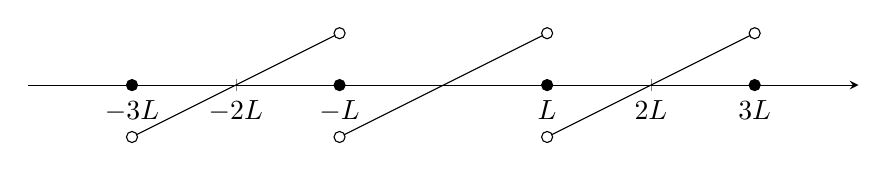
\begin{tikzpicture}
    \begin{axis}[axis x line=middle, axis y line=middle, xtick = {-3,-2,-1,1,2,3}, xticklabels={$-3L$,$-2L$,$-L$,$L$,$2L$,$3L$}, ymax=1, ymin=-1, xmax=4, xmin=-4,width=\textwidth, hide y axis,unit vector ratio=2]
  
    \addplot[mark=*] coordinates {(-1,0)};
    \addplot[mark=*] coordinates {(1,0)};
    \addplot[mark=*] coordinates {(-3,0)};
    \addplot[mark=*] coordinates {(3,0)};
    \addplot[mark=*,fill=white] coordinates {(1,1)};
    \addplot[mark=*,fill=white] coordinates {(3,1)};
    \addplot[mark=*,fill=white] coordinates {(-1,-1)};
    \addplot[mark=*,fill=white] coordinates {(1,-1)};
    \addplot[mark=*,fill=white] coordinates {(-1,1)};
    \addplot[mark=*,fill=white] coordinates {(-3,-1)};
    \addplot[domain=-1:1] {x};
    \addplot[domain=1:3] {x-2};
    \addplot[domain=-3:-1] {x+2};
    \end{axis}
    \end{tikzpicture}

\end{answer}
\newpage
\begin{exer} 

\end{exer}
\begin{answer}


\begin{align*}
    \textbf{(A)}
\end{align*}
Yes, If $f(x)$ has a Fourier series representation, then that Fourier series converges to $f(x)$ at all but countably many points. It is also bounded. Any bounded function with countably many discontinuities is integrable. 

\end{answer}

\newpage


\begin{exer} 

\end{exer}
\begin{answer}


\begin{align*}
    \textbf{(A)}
\end{align*}
 Not necessarily. 
\begin{align*}
    \textbf{(B)}
\end{align*}

For example, taking $L=\pi$ for simplicity, we attempt to differentiate, term-by-term, the Fourier series from problem 4 and compare that to what we know about $f'(x)$  

\begin{align*}
    \sum_{n=1}^{\infty} \Big(\frac{2(-1)^{n+1}}{n }\Big)\Big(\sin\big( n x\big)\Big)' = \sum_{n=1}^{\infty}2(-1)^{n+1}\cos(nx).
\end{align*}
We know that $f'(x) = 1 $ for all $x$, including $x=\pi$. However, our term-by-term differentiation at $x=\pi$ becomes
\begin{align*}
    \sum_{n=1}^{\infty}2(-1)^{n+1}(-1)^n = 2\sum_{n=1}^{\infty}(-1)^{2n+1}= 2\sum_{n=1}^{\infty}(-1)
\end{align*}
This is a divergent series. This comports with Theorem 2.13, which tell us that we can differentiate a Fourier series representation term-by-term if the function is continuous, and this function has a jump discontinuity. 
\end{answer}

\end{document}
 